\documentclass[Main]{subfiles}

\begin{document}

\chapter{Scope}

\section{Identification}
This System Test Description(STD) identifies, specifies and establishes the detailed test description for the Self Protection Suite.
The STD specifies the methods to be used to ensure that each requirement has been met. 

\section{System overview}
The purpose of the SPS is to provide Royal Danish Air Force with a self-protection suite for the F-16 combat aircraft which will dispense payloads and host a Missile Warning System. 
The system will provide warning upon detection of missile threats and automatically dispense payloads in response.

\begin{figure}[H]
\centering
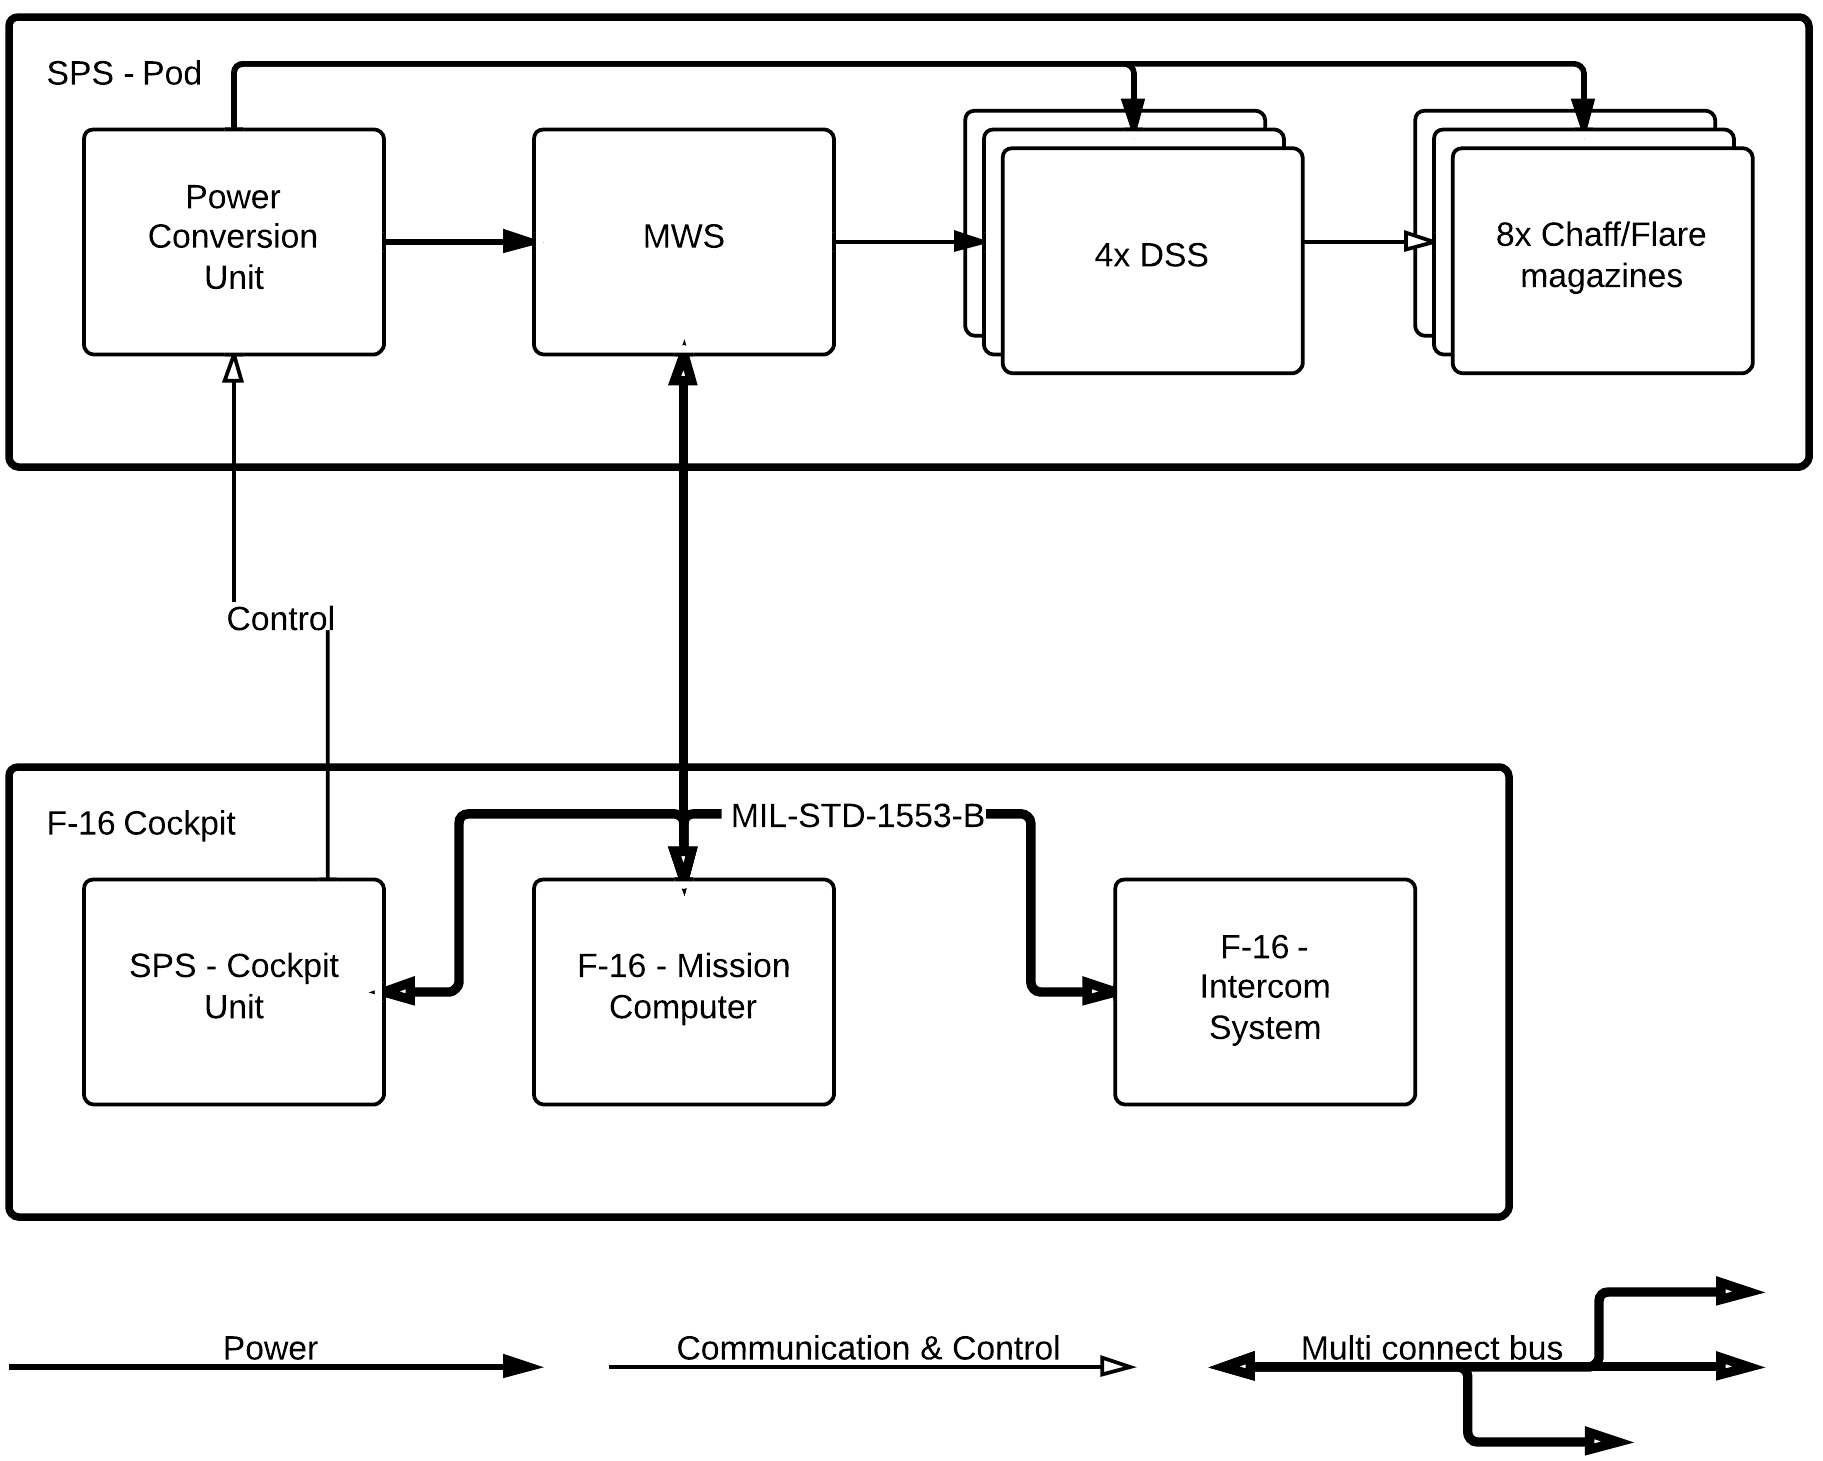
\includegraphics[width = 0.9\textwidth]{ConceptOfOperations}
\caption{Concept of operations}
\end{figure}


\section{Document overview}
This section has been tailored out. See Table of Contents.



\end{document}